\section{Durchführung}
\label{sec:Durchführung}
Die Messapparatur vor Ort ist nach dem Schema in \autoref{fig:aufbauschema} aufgebaut.
\begin{figure}
    \centering
    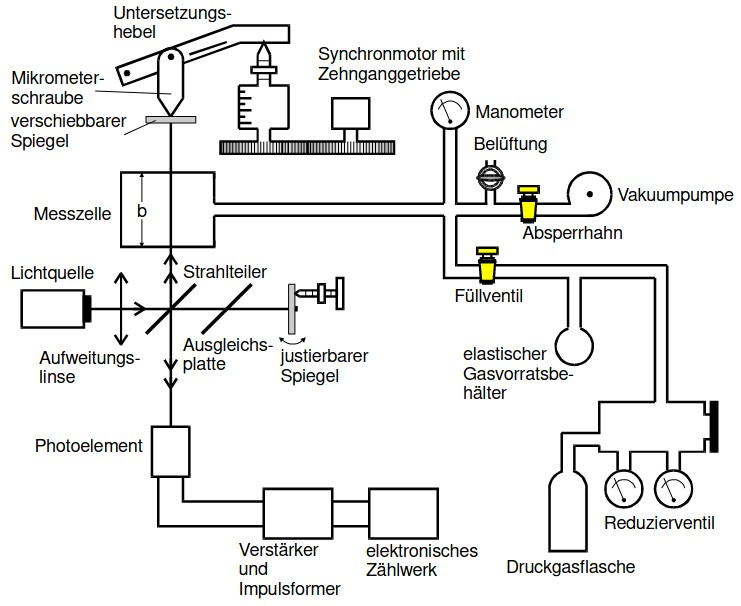
\includegraphics[width=\textwidth]{content/aufbauversuch.jpg}
    \caption{Der schematische Aufbau der Messapparatur vor Ort.}
    \label{fig:aufbauschema}
\end{figure}

\noindent
Nachdem der Raum vollständig abgedunkelt wird, damit keine Änderung der Lichtverhältnisse das Messergebnis verfälschen kann, wird das Interferometer einjustiert.
Dafür wird vor den Detektor eine Mattscheibe gehalten und die am hellsten zu sehenden Punkte werden zur Deckung gebracht. Außerdem wird die als Detektor verwendete
Photozelle so ausgerichtet, dass das Interferenzbild genau auf den Eintrittsspalt fällt.


\subsection{Bestimmung der Wellenlänge des Lasers}
Nun kann die Messung zur Bestimmung der Wellenlänge des Lasers begonnen werden. Dafür wird mit Hilfe eines Motors und einer Mikrometerschraube der verschiebbare 
Spiegel jeweils um $\SI{5}{\milli\meter}$ bewegt und die in diesem Vorgang durchlaufenden Maxima gezählt. Das Zählen der durchlaufenden Maxima wird von der 
Photozelle übernommen. Es ist wichtig, darauf zu achten, dass der Spiegel nicht zu schnell verschoben wird, da sonst nicht alle Maxima detektiert werden können.
Es wird darauf geachtet, dass die Mikrometerschraube auf 0 steht und dann vom Motor auf $\SI{5}{\milli\metre}$ gedreht wird. Die bei dieser Bewegung durchlaufende
Maximaanzahl wird notiert. Die Schraube wird etwas weiter aufgedreht, um anschließend den Spiegel um $\SI{5}{\milli\meter}$ zurück zu bewegen. Auch hier werden die Maximaanzahl notiert.
Dieser Messvorgang wird fünf mal wiederholt, sodass 10 Wertepaare aufgenommen werden.

\subsection{Bestimmung des Brechungsindexes von Luft}
Zur Bestimmung des Brechungsindexes wird der Aufbau des Experimentes nicht verändert. In einer der beiden Strecken befindet sich eine Messzelle, welche mit Luft gefüllt ist.
Nun wird die Anzahl der durchlaufenden Maxima gezählt, während mit einer Vakuumpumpe bis zu einer gewissen Druckanzahl die Luft aus der Messzelle gepumpt wird.
Dann wird langsam die Luft wieder in die Messzelle gelassen; hierbei wird auch nochmal die Maximaanzahl notiert. Es ist hier sehr wichtig, schnell den Wert zu notieren und die Luft einströmen zu lassen, 
da der erreichte Druck von der Messapparatur nicht lange gehalten wird. Der Messvorgang wird einige Male wiederholt.

\begin{figure}
    \centering
    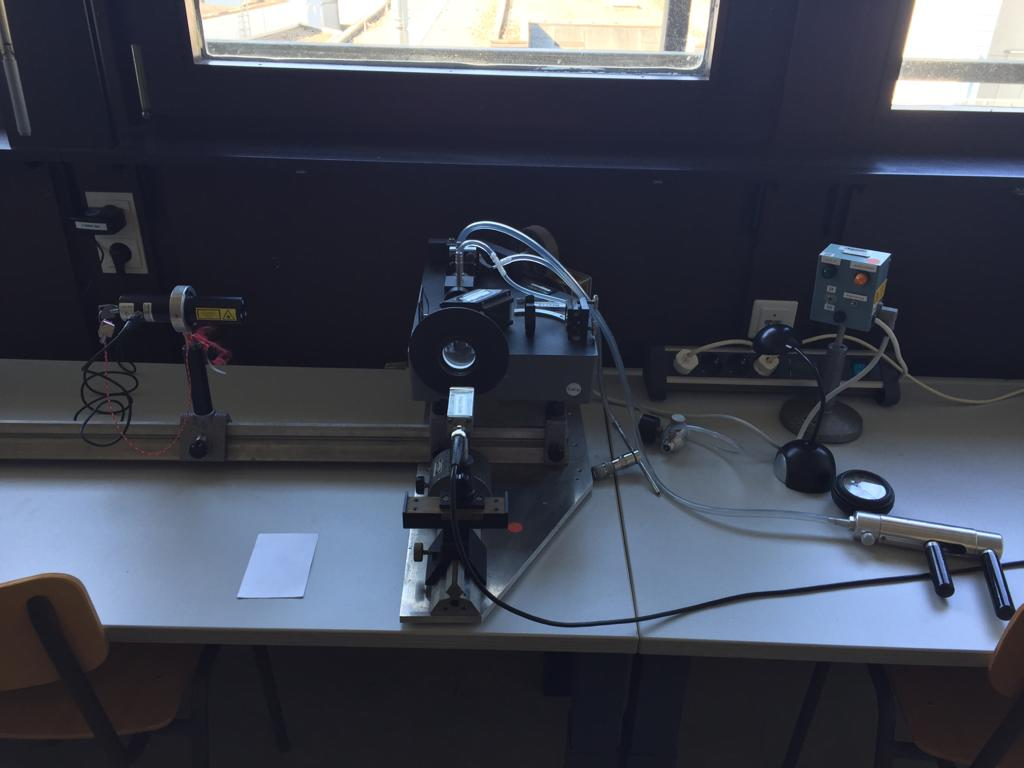
\includegraphics[width=0.6\textwidth]{content/aufbaufoto1.jpeg}
    \caption{Der Versuchsaufbau vor Ort. Links ist der Laser zu sehen, welcher auf den semipermeablen Spiegel gerichtet ist. Hinter den Schläuchen ist der verstellbare
    Spiegel und der Motor zu erkennen. Der Spiegel rechts auf der Apparatur hat die Schrauben zum Justieren. Vor der Apparatur ist die Zestrungslinse und der Detektor.
    Der bläuliche Kasten beinhaltet die Schalter für den Motor und die Schläuche verbinden die Messzelle auf der Apparatur mit dr Vakuumpumpe auf dem Tisch.}
\end{figure}

\begin{figure}
    \centering
    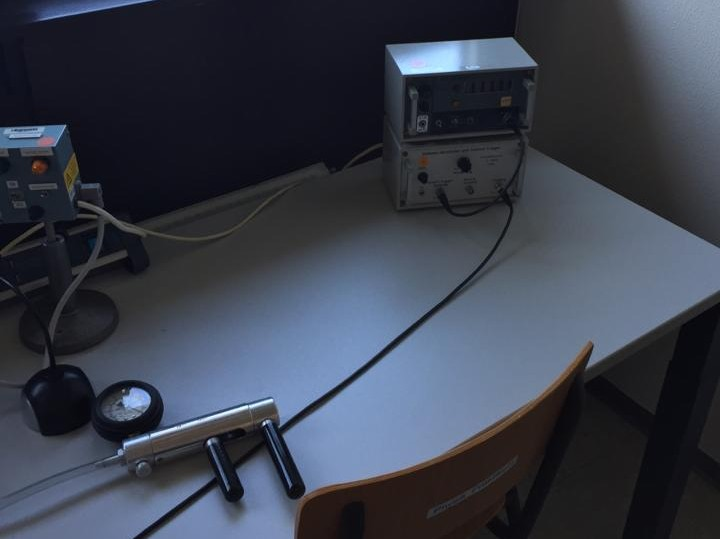
\includegraphics[width=0.6\textwidth]{content/aufbaufoto2.jpeg}
    \caption{Hier ist der Impulszähler auf dem Selektivverstärker zu sehen.}
\end{figure}